%% beamer packages
% other themes: AnnArbor, Antibes, Bergen, Berkeley, Berlin, Boadilla, boxes, 
% CambridgeUS, Darmstadt, Dresden, Frankfurt, Goettingen, Hannover, Ilmenau,
%JuanLesPins, Luebeck, Madrid, Malmoe, Marburg, Montpellier, PaloAlto,
%Pittsburgh, Rochester, Singapore, Szeged, Warsaw
% other colors: albatross, beaver, crane, default, dolphin, dove, fly, lily, 
%orchid, rose, seagull, seahorse, sidebartab, structure, whale, wolverine,
%beetle

%\documentclass[xcolor=dvipsnames]{beamer}
\documentclass[table,dvipsnames]{beamer}
\usepackage{beamerthemesplit}
\usepackage{bm,amsmath,marvosym}
\usepackage{listings,color}%xcolor
\usepackage[ngerman]{babel}
\usepackage{natbib}
\usepackage[utf8]{inputenc}
\definecolor{shadecolor}{rgb}{.9, .9, .9}
\definecolor{darkblue}{rgb}{0.0,0.0,0.5}
\definecolor{myorange}{cmyk}{0,0.7,1,0}
\definecolor{mypurple}{cmyk}{0.3, 0.9, 0.0, 0.2}

% make a checkmark
\usepackage{tikz}
\def\checkmark{\tikz\fill[scale=0.4](0,.35) -- (.25,0) -- (1,.7) -- (.25,.15) -- cycle;} 

% dot product
\usetikzlibrary{arrows,positioning}
\tikzset{
    %Define standard arrow tip
    >=stealth',
    % Define arrow style
    pil/.style={->,thick}
}

% math stuff
\newcommand{\argmin}{\operatornamewithlimits{argmin}}

\lstnewenvironment{code}{
    \lstset{backgroundcolor=\color{shadecolor},
        showstringspaces=false,
        language=python,
        frame=single,
        framerule=0pt,
        keepspaces=true,
        breaklines=true,
        basicstyle=\ttfamily,
        keywordstyle=\bfseries,
        basicstyle=\ttfamily\scriptsize,
        keywordstyle=\color{blue}\ttfamily,
        stringstyle=\color{red}\ttfamily,
        commentstyle=\color{green}\ttfamily,
        columns=fullflexible
    }
}{}

\lstnewenvironment{codeout}{
    \lstset{backgroundcolor=\color{shadecolor},
        frame=single,
        framerule=0pt,
        breaklines=true,
        basicstyle=\ttfamily\scriptsize,
        columns=fullflexible
    }
}{}

\hypersetup{colorlinks = true, linkcolor=darkblue, citecolor=darkblue,urlcolor=darkblue}
\hypersetup{pdfauthor={A. Richards}, pdftitle={Projects}}

\newcommand{\rd}{\textcolor{red}}
\newcommand{\grn}{\textcolor{green}}
\newcommand{\keywd}{\textcolor{myorange}}
\newcommand{\highlt}{\textcolor{darkblue}}
\newcommand{\norm}[1]{\left\lVert#1\right\rVert}
\def\ci{\perp\!\!\!\perp}
% set beamer theme and color
\usetheme{Frankfurt}
%\usetheme{Berkeley}
\usecolortheme{orchid}
%\usecolortheme{seagull}
\setbeamertemplate{blocks}[rounded][shadow=true]

\title[Project teams]{Python and Data Science \\ (Live Coding)}
\author[Galvanize DS]{A. Richards}
\institute{}
\date[]{09.13.2017}

%%%%%%%%%%%%%%%%%%%%%%%%%%%%%%%%%%%%%%%%%%%%%%%%%%%%%%%%%%%%%%%%%%%%%%%%%%%%%%%
\begin{document}
\frame{\titlepage}
%%%%%%%%%%%%%%%%%%%%%%%%%%%%%%%%%%%%%%%%%%%%%%%%%%%%%%%%%%%%%%%%%%%%%%%%%%%%%%%
\frame{
\footnotesize
\tableofcontents
\normalsize
}

%%%%%%%%%%%%%%%%%%%%%%%%%%%%%%%%%%%%%%%%%%%%%%%%%%%%%%%%%%%%%%%%%%%%%%%%%%%%%%%
\section{Why.. Why?}
\subsection{}
%%%%%%%%%%%%%%%%%%%%%%%%%%%%%%%%%%%%%%%%%%%%%%%%%%%%%%%%%%%%%%%%%%%%%%%%%%%%%%%
\frame{   
\frametitle{Why Data Science?}
\footnotesize
\begin{block}{Well because of the \keywd{data} and because of the \keywd{science}}
 \begin{itemize}
    \item Data science means different things to different people
    \begin{itemize}
         \item Data engineering $\rightarrow$ data vis $\rightarrow$ predictive modeling
    \end{itemize}
    \item Statistics, machine-learning, databases, web-development
    \item We are in an era of unprecedented data growth
    \begin{itemize}
        \item And so few know how to effectively use data to gain insight
    \end{itemize}
    \item Science is the proponent of truth through the communication of evidence
    \end{itemize}
\end{block}

\visible<2->{
\begin{block}{}
\keywd{There are jobs as well!}
\end{block}
}
}

%%%%%%%%%%%%%%%%%%%%%%%%%%%%%%%%%%%%%%%%%%%%%%%%%%%%%%%%%%%%%%%%%%%%%%%%%%%%%%%
\frame{   
\frametitle{The essential data science toolkit}
\begin{block}{Subject area mastery}
 \begin{itemize}
    \item SQL and noSQL databases
    \item Associative statistics and hypothesis testing
    \item Unsupervised and supervised learning
    \item Data visualization
    \item Data products
    \end{itemize}
\end{block}

\begin{block}{Programming mastery}
 Expert level proficiency in language that is useful for data science 
\end{block}
}

%%%%%%%%%%%%%%%%%%%%%%%%%%%%%%%%%%%%%%%%%%%%%%%%%%%%%%%%%%%%%%%%%%%%%%%%%%%%%%%
\frame{   
\frametitle{Why Python?}
\begin{block}{}
\begin{itemize}
    \item There are many languages of data science (Python, R,...)
    \item Ecosystem (NumPy, matplotlib, pandas)
    \item Readability, Flexibility
    \item Glue language
    \item Object-oriented and functional
    \end{itemize}
\end{block}
}


%%%%%%%%%%%%%%%%%%%%%%%%%%%%%%%%%%%%%%%%%%%%%%%%%%%%%%%%%%%%%%%%%%%%%%%%%%%%%%%
\section{nlp}
\subsection{}

%%%%%%%%%%%%%%%%%%%%%%%%%%%%%%%%%%%%%%%%%%%%%%%%%%%%%%%%%%%%%%%%%%%%%%%%%%%%%%%
\frame{
\frametitle{What is NLP?}
\scriptsize
\begin{center}
 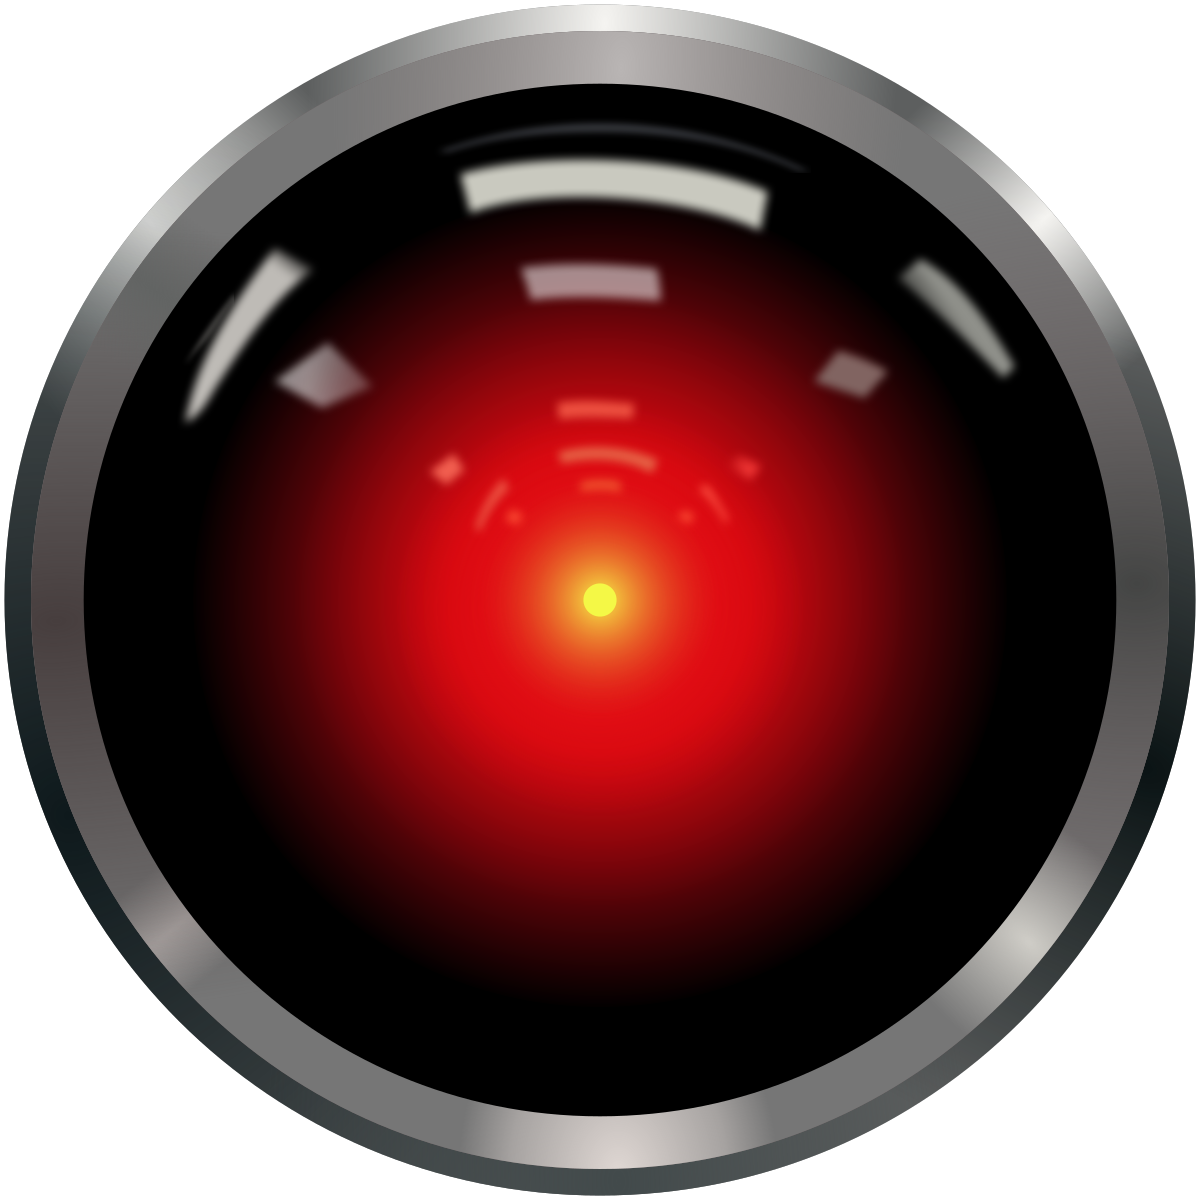
\includegraphics[scale=0.05]{hal.png}
\end{center}

\begin{itemize}
  \item \highlt{Conversational Agents}
  \begin{itemize}
   \item Siri, Cortana, Google Now, Alexa
   \item Talking to your car
   \item Communicating with robots
  \end{itemize}

  \item \highlt{Machine Translation} 
  \begin{itemize}
  \item Google Translate
  \item \href{https://research.google.com/pubs/pub45610.html}{Google's Neural Machine Translation}
  \end{itemize}
  \item Speech Recognition, Speech Synthesis
  \item Lexical Semantics, Sentiment Analysis 
  \item Dialogue Systems, Question Answering
\end{itemize}

\begin{flushleft}
\begin{tiny}
\href{https://web.stanford.edu/class/cs124/lec/chatbot.pdf}{Conversation Agent Lecture - Dan Jurafsky}
\end{tiny}
\end{flushleft}
}

%%%%%%%%%%%%%%%%%%%%%%%%%%%%%%%%%%%%%%%%%%%%%%%%%%%%%%%%%%%%%%%%%%%%%%%%%%%%%%%
\frame{
\frametitle{NLP and AI}
\scriptsize
\begin{block}{}
The ultimate goal of NLP is to the fill the gap how the humans communicate (natural language) and what the computer understands (machine language).
\end{block}
\begin{center}
 
\includegraphics[scale=0.3]{ai-enabled-systems.png}
\end{center}

Why Deep Learning Needed in NLP

 \begin{itemize}
  \item It uses a rule-based approach that represents Words as ‘One-Hot’ encoded vectors.
  \item Traditional method focuses on syntactic representation instead of semantic representation.
  \item Bag of words - classification model is unable to distinguish certain contexts.
\end{itemize}

\begin{flushleft}
\begin{tiny}
\href{http://www.datasciencecentral.com/profiles/blogs/overview-of-artificial-intelligence-and-role-of-natural-language}{http://www.datasciencecentral.com/profiles/blogs/overview-of-artificial-intelligence-and-role-of-natural-language}
\end{tiny}
\end{flushleft}
}

%%%%%%%%%%%%%%%%%%%%%%%%%%%%%%%%%%%%%%%%%%%%%%%%%%%%%%%%%%%%%%%%%%%%%%%%%%%%%%%
\frame{ 
\begin{center}
 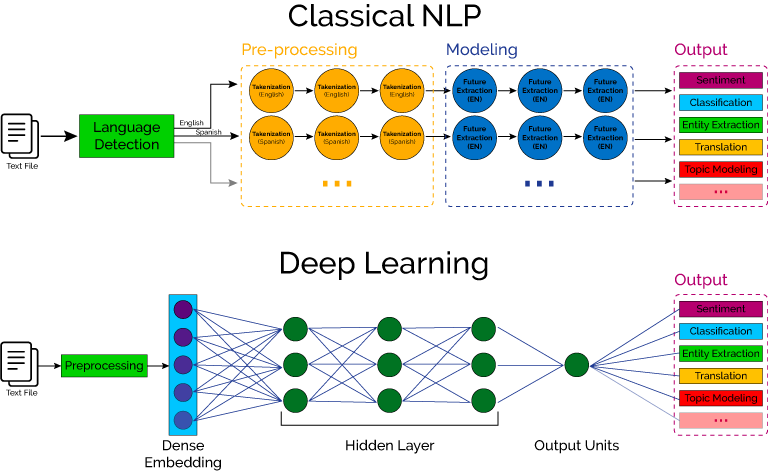
\includegraphics[scale=0.4]{difference-between-classical-nlp-deep-learning-nlp.png}
\end{center}
\begin{flushleft}
\begin{tiny}
\href{blog.aylien.com}{blog.aylien.com}
\end{tiny}
\end{flushleft}
}

%%%%%%%%%%%%%%%%%%%%%%%%%%%%%%%%%%%%%%%%%%%%%%%%%%%%%%%%%%%%%%%%%%%%%%%%%%%%%%%
\frame{ 

\begin{block}{What is the meaning of this sentence?}
\ \\
\begin{center}I made her duck.\end{center}
\ \\
\end{block}
}

%%%%%%%%%%%%%%%%%%%%%%%%%%%%%%%%%%%%%%%%%%%%%%%%%%%%%%%%%%%%%%%%%%%%%%%%%%%%%%%
\frame{ 
\frametitle{Challenges}
\footnotesize

\keywd{Ambiguity} \ \\
What does it mean when we say: \highlt{`I made her duck'}
 \begin{itemize}
   \item I cooked waterfowl for her
   \item I cooked waterfowl belonging to her
   \item I created the (papier mache?) duck she owns
   \item I caused her to quickly lower her head or body
   \item I waved my magic wand and turned her into undifferentiated waterfowl
\end{itemize}

\keywd{Other examples}
\begin{itemize}
 \item `Court to try shooting defendant'
 \item `Hospitals are sued by seven foot doctors'
\end{itemize}
 
This problem of determining which sense was meant by a specific word is formally known as \keywd{word sense disambiguation}

Other challenges include:
\begin{itemize}
 \item Part of speech tagging 
 \item Syntactic disambiguation (The I made her duck example)
\end{itemize}

\begin{flushleft}
 \begin{tiny}
  Speech and Language Processing (Jurafsky and Martin)
 \end{tiny}
\end{flushleft}
}

%%%%%%%%%%%%%%%%%%%%%%%%%%%%%%%%%%%%%%%%%%%%%%%%%%%%%%%%%%%%%%%%%%%%%%%%%%%%%%%
\section{Demos}
\subsection{}

%%%%%%%%%%%%%%%%%%%%%%%%%%%%%%%%%%%%%%%%%%%%%%%%%%%%%%%%%%%%%%%%%%%%%%%%%%%%%%%
\frame{   
\frametitle{Demo 1}
\begin{block}{}
 Tutorial Example
\end{block}
}


%%%%%%%%%%%%%%%%%%%%%%%%%%%%%%%%%%%%%%%%%%%%%%%%%%%%%%%%%%%%%%%%%%%%%%%%%%%%%%%
\frame{ 
\begin{center}
 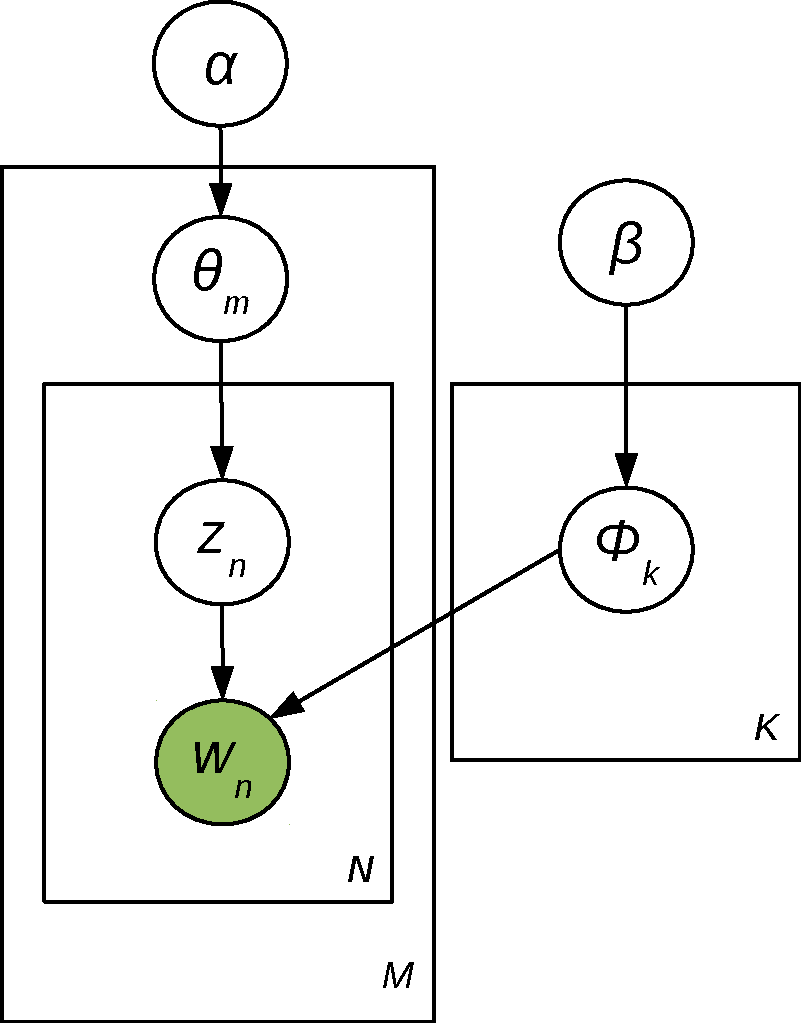
\includegraphics[scale=0.3]{lda_plate.pdf}
\end{center}
}



%%%%%%%%%%%%%%%%%%%%%%%%%%%%%%%%%%%%%%%%%%%%%%%%%%%%%%%%%%%%%%%%%%%%%%%%%%%%%%%
\frame{   
\frametitle{Demo 2}
\begin{block}{}
 Advanced Example
\end{block}
}

%%%%%%%%%%%%%%%%%%%%%%%%%%%%%%%%%%%%%%%%%%%%%%%%%%%%%%%%%%%%%%%%%%%%%%%%%%%%%%%
\section{Discussion and Wrap-up}
\subsection{}

%%%%%%%%%%%%%%%%%%%%%%%%%%%%%%%%%%%%%%%%%%%%%%%%%%%%%%%%%%%%%%%%%%%%%%%%%%%%%%%
\frame{   
\frametitle{Overview}
\begin{block}{}
 \begin{enumerate}
    \item Version control based workflow
    \item Jupyter notebook
    \item Data types (lists, arrays, data frames)
    \item EDA - working with data frames, plotting
    \item Working with text (latent topics, clustering)
    \item Data visualization
    \end{enumerate}
\end{block}
}

%%%%%%%%%%%%%%%%%%%%%%%%%%%%%%%%%%%%%%%%%%%%%%%%%%%%%%%%%%%%%%%%%%%%%%%%%%%%%%%
\frame{   
\footnotesize
\begin{table}
\begin{tabular}{|c|c|}
\hline
Week& Topic \\
\hline
0   & Python workshop \\
1   & Programming and SQL \\
2   & Probability and Statistics \\
3   & Linear Models \\
4   & Supervised Learning \\
5   & NLP, Business analytics \\
6   & Unsupervised Learning \\
7   & Break Week \\
8   & Big Data / Data Engineering \\
9   & Special Topics / Case Studies \\
9   & Project \\
10  & Project \\
11  & Project \\
12  & Career services and Special topics \\
\hline
\end{tabular}
\end{table}

There are also part-time courses and free meet-ups...
}


\end{document}